\section{Mapping Instructions and Visual Observations to Actions~\cite{DBLP:journals/corr/MisraLA17}}
They propose to directly map raw visual observations and text input to actions for instruction execution.  While existing approaches assume access to structured environment representations or use a pipeline of separately trained models, they learn a single model to jointly reason about linguistic and visual input. They use reinforcement learning in a contextual bandit setting to train a neural network agent. To guide the agent’s exploration, they use reward shaping with different forms of supervision~\cite{DBLP:journals/corr/MisraLA17}.

\begin{figure}[htbp]
    \centering
    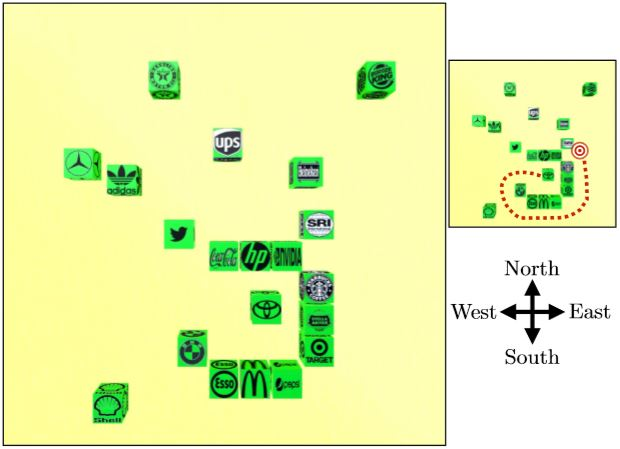
\includegraphics[width=.8\textwidth]{block}
    \caption{Blocks environment}
\end{figure}
\newpage
\begin{table}[h!]
    \begin{tabular}{|p{15cm}|}
    \hline
    Put the Toyota block in the same row as the SRI block, in the first open space to the right of the SRI block.\\
    \hline
    Move Toyota to the immediate right of SRI, evenly aligned and slightly separated.\\
    \hline
    Move the Toyota block around the pile and place it just to the right of the SRI block.\\
    \hline
    Place Toyota block just to the right of The SRI Block.\\
    \hline
    Toyota, right side of SRI.\\
    \hline
    \end{tabular}
    \caption{Instructions in the Blocks environment}
    \label{tab:1}
\end{table}

In Table~\ref{tab:1}, illustrates the problem in the Blocks environment. The agent observes the environment as an RGB image using a camera sensor. Given the RGB input, the agent must recognize the blocks and their layout. To understand the instruction, the agent must identify the block to move (Toyota block) and the destination (just right of the SRI block). This requires solving semantic and grounding problems. For example, consider the topmost instruction in the figure. The agent needs to identify the phrase referring to the block to move, Toyota block, and ground it. It must resolve and ground the phrase SRI block as a reference position, which is then modified by the spatial meaning recovered from the same row as or first open space to the right of, to identify the goal position. Finally, the agent needs to generate actions, for example moving the Toyota block around obstructing blocks. 

To address these challenges with a single model, they design a neural network agent. The agent executes instructions by generating a sequence of actions. At each step, the agent takes as input the instruction text, observes the world as an RGB image, and selects the next action. Action execution changes the state of the world. Given an observation of the new world state, the agent selects the next action. This process continues until the agent indicates execution completion. When selecting actions, the agent jointly reasons about its observations and the instruction text. This enables decisions based on close interaction between observations and linguistic input.

They study the problem of learning to execute instructions in a situated environment given only raw visual observations. Supervised approaches do not explore adequately to handle test time errors, and reinforcement learning approaches require a large number of samples for good convergence. Their solution provides an effective combination of both approaches: reward shaping to create relatively stable optimization in a contextual bandit setting.

This combination is designed for a few-samples regime, as we address. When the number of samples is unbounded, the drawbacks observed in this scenario for optimizing longer term reward do not hold.
